%\documentclass[spanish]{article}
\documentclass[12pt,a4paper,spanish]{book}
\usepackage[spanish]{babel}
\usepackage[utf8]{inputenc}
\usepackage[T1]{fontenc}
\usepackage{amsmath}
\usepackage{amsthm}
\usepackage{amsfonts}
\usepackage{amssymb}
\usepackage{shadow}
\usepackage{indentfirst}
\usepackage{fancyhdr}
\linespread{1.25}
\usepackage{graphicx}
\usepackage{pdfpages}
\usepackage{subfigure}
\usepackage{framed}
\usepackage{array}
\usepackage{appendix}
\usepackage[bookmarks=true,bookmarksopen,hidelinks,bookmarksdepth=3,colorlinks=false]{hyperref}
\usepackage{graphics}
\usepackage{anysize}
\usepackage{theorem}
\usepackage{float}
\marginsize{4cm}{2cm}{2cm}{2cm}
\usepackage[Glenn]{fncychap}
\usepackage{url}
\usepackage{multicol}
\usepackage{awesomebox}
\pagestyle{fancy}
\usepackage{titling}
\usepackage{lastpage}
\usepackage{lipsum}  
\usepackage{fancyhdr}
\usepackage{extramarks}
\usepackage{float}
\usepackage{flowchart}
\usetikzlibrary{arrows}
\usepackage{etoolbox}
\AtBeginEnvironment{tikzpicture}{\shorthandoff{>}\shorthandoff{<}}{}{}
\usepackage[acronym,nonumberlist,shortcuts,sanitize=none,nomain]{glossaries}
\makeglossaries
\usepackage[xindy]{imakeidx}
\makeindex
\usepackage{color}
\definecolor{gray97}{gray}{.97}
\definecolor{gray75}{gray}{.75}
\definecolor{gray45}{gray}{.45}
\definecolor{javared}{rgb}{0.6,0,0}
\definecolor{javagreen}{rgb}{0.25,0.5,0.35}
\definecolor{javapurple}{rgb}{0.5,0,0.35}
\definecolor{javadocblue}{rgb}{0.25,0.35,0.75}
\definecolor{OliveGreen}{rgb}{0,0.6,0}

\usepackage{minted}
\usemintedstyle{emacs}

\newacronym{APK}{APKs}{Android Application Package}

\newglossaryentry{JDK}{
first={Java Development Kit},
name={JDK},
description={Conjunto oficial de herramientas necesarias para el desarrollo de aplicaciones en Java.},
sort={JDK}
}


\newcommand{\lsidequotesize}{40}
\newcommand{\lsidequotecoeff}{0.325}
\definecolor{quotemarkcolor}{rgb}{0.5,0.5,0.5}

\reversemarginpar
\usepackage[colorinlistoftodos,prependcaption,textsize=tiny]{todonotes}

\newcommand{\unsure}[1]{\todo[linecolor=red,backgroundcolor=red!25,bordercolor=red]{#1}}
\newcommand{\change}[1]{\todo[linecolor=blue,backgroundcolor=blue!25,bordercolor=blue]{#1}}
\newcommand{\info}[1]{\todo[linecolor=OliveGreen,backgroundcolor=OliveGreen!25,bordercolor=OliveGreen]{#1}}
\newcommand{\improvement}[1]{\todo[linecolor=Plum,backgroundcolor=Plum!25,bordercolor=Plum]{#1}}


\newcommand{\rulesep}{\unskip\ \vrule\ }

\usepackage{caption}
\usepackage{subcaption}
\captionsetup[figure]{labelfont=it,textfont={it}}
\captionsetup[subfigure]{labelfont=bf,textfont=normalfont,singlelinecheck=off,justification=raggedright}

\tolerance=1
\emergencystretch=\maxdimen
\hyphenpenalty=10000
\hbadness=10000

\usepackage[style=alphabetic]{biblatex}
\addbibresource{Extra/Bibliografia.bib}


\raggedbottom
\begin{document}

\DeclareGraphicsExtensions{.jpg,.pdf,.mps,.png,.gif,.fig,.bmp, .PNG}

%===================================
% Definición de campos.
%===================================

\title{Este es el título.}
  
\author{AUTOR 1, AUTOR 2}

\newcommand{\asignatura}{Esta es la asignatura}


%===================================
% Acta
%===================================
%\thispagestyle{empty}
%\includepdf[pages=1]{Acta/acta.pdf} %%% Ya que el acta tiene un formato específico, se crea un pdf a partir de un fichero de word y se incluye %%%
%\newpage
%\thispagestyle{empty}\cleardoublepage

%===================================
% Portada
%===================================

%%Portada%%
%====
%------- TÍTULO     ----------
%=============================

\pretitle{
	\begin{center}
    \LARGE
    
\includegraphics[scale=1]{Portada/logotipo_MDS.png}
    \vspace{0.5cm}\\
    \textbf{Máster en Data Science. URJC}\\
	\textbf{\asignatura}\\	
    \vspace{0.5cm}}
\posttitle{
	\end{center}
}


\preauthor{
	\begin{center}
	\fontsize{14bp}{14bp}\selectfont
}
\postauthor{\par\end{center}\vspace{24bp}}
\maketitle


\renewcommand\tablename{Tabla}
\renewcommand\listfigurename{Lista de Figuras}
\renewcommand\listtablename{Lista de Tablas}

\thispagestyle{empty} \cleardoublepage


%===================================
%Cita
%===================================
\thispagestyle{empty}
\newpage
\bigskip
\bigskip
\begin{flushright}
\emph{La utopía está en el horizonte.Camino dos pasos, ella se aleja dos pasos y el horizonte se corre diez pasos más allá. ¿Entonces para que sirve la utopía? Para eso, sirve para caminar.}\\
Eduardo Galeano.

\medskip

\emph{El software es como el sexo: mejor si es libre y gratis.}\\
Linus Torvalds.
\end{flushright}

\newpage
\thispagestyle{empty}\cleardoublepage

%===================================
%Dedicatoria
%===================================
\thispagestyle{empty}
\newpage
\bigskip
\bigskip
\begin{flushright}
  Dedicado a Monstruo de Espagueti Volador.
\end{flushright}

\newpage
\thispagestyle{empty}\cleardoublepage

%===================================
%Agradecimientos
%===================================
\frontmatter
\thispagestyle{plain}
\chapter*{Agradecimientos}
\addcontentsline{toc}{chapter}{Agradecimientos}
\markboth{AGRADECIMIENTOS}{AGRADECIMIENTOS}

Agradecerselo a Son Goku, quien dío varias veces su vida para asegurar el futuro de la humanidad.
\cleardoublepage


%====================================
%		Para el encabezado que se va a utilizar en todo el proyecto
%====================================
\pagestyle{fancy}

\renewcommand{\sectionmark}[1]{\markright{\thesection\ #1}}
\fancyhf{}
\fancyhead[RE]{\leftmark}
\fancyhead[LO]{\rightmark}}
\fancyhead[RO]{
\includegraphics[width=0.5cm,height=0.5cm]{Portada/DSLab_logo_2.png}}
\fancyfoot[LE]{\thepage}
\fancyfoot[RE]{Máster en Data Science. URJC, 2018}
\fancyfoot[LO]{\asignatura}
\fancyfoot[RO]{\thepage}

%===================================
%Resumen
%===================================
\chapter*{Resumen}
\addcontentsline{toc}{chapter}{Resumen}
\markboth{RESUMEN}{RESUMEN}

Bla Bla Bla Bla Bla
\cleardoublepage

%===================================
%Abstract
%===================================
\chapter*{Abstract}
\addcontentsline{toc}{chapter}{Abstract}
\markboth{ABSTRACT}{ABSTRACT}

Bla Bla Bla Bla pero en inglés.
\cleardoublepage

%====================================
%Índices
%====================================

\setcounter{secnumdepth}{3}
\setcounter{tocdepth}{3}
\tableofcontents
\addcontentsline{toc}{chapter}{Lista de figuras}
\listoffigures


%============================================================
%   Glosario
%============================================================
\renewcommand*{\acronymname}{Glosario}
\renewcommand*{\glossaryname}{Glosario}
\deftranslation{Glossary}{Glosario}
\addcontentsline{toc}{section}{Glosario}
\markboth{GLOSARIO}{GLOSARIO}
\printglossaries


%=============================================================
%		Contenido
%=============================================================
\mainmatter
\chapter{Capítulo}

\lipsum[1]

\section{Sección}

\lipsum[1]

\subsection{Algunas cosillas}


\subsubsection{Referencias}

Para referenciar a una palabra del glosario

\glsfirst{JDK} \\
\gls{APK} \\
\gls{JDK} \\
\cite{AngBenNadel}

\subsubsection{Imagen}

\begin{figure}[H]
\centering
  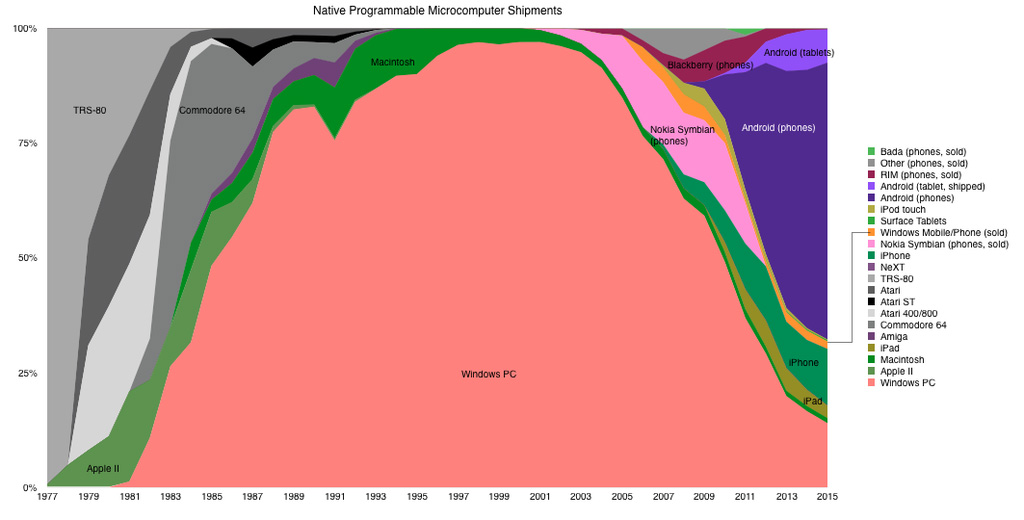
\includegraphics[width=\textwidth]{Figures/ch1/introduction/os_quota}
  \caption{Pie de imagen. }
\end{figure}

\subsubsection{Código}

Bash


\begin{minted}[
frame=lines,
linenos
]{bash}
    cd
    ls
    echo "Hello World"
\end{minted}

Python


\begin{minted}[
frame=lines,
linenos
]{python}
import os
class HelloWorld:
    msg = "Hello World"
    def __init__(self):
        print(self.msg)

if __name__ == '__main__':
    HelloWorld()	
\end{minted}


\chapter*{Conclusiones}
\addcontentsline{toc}{chapter}{Conclusiones}
\markboth{CONCLUSIONES}{CONCLUSIONES}

\lipsum

%------------------------------------------------------------
%          Bibliografia
%------------------------------------------------------------
\cleardoublepage
\addcontentsline{toc}{chapter}{Bibliografía}
\printbibliography

%============================================================
%   Apéndices
%============================================================
\renewcommand{\appendixtocname}{ANEXOS}
\renewcommand{\appendixpagename}{ANEXOS}
\renewcommand{\appendixname}{ANEXOS}
\appendix
\appendixpage
\addappheadtotoc
\begin{appendices}
\addtocontents{toc}{\protect\setcounter{tocdepth}{5}}
\chapter{Anexo I}
\lipsum


\end{appendices}

\end{document}
